\let\negmedspace\undefined
\let\negthickspace\undefined
\documentclass[journal,12pt,twocolumn]{IEEEtran}
\usepackage{cite}
\usepackage{amsmath,amssymb,amsfonts,amsthm}
\usepackage{algorithmic}
\usepackage{graphicx}
\usepackage{textcomp}
\usepackage{xcolor}
\usepackage{txfonts}
\usepackage{listings}
\usepackage{enumitem}
\usepackage{mathtools}
\usepackage{gensymb}
\usepackage[breaklinks=true]{hyperref}
\usepackage{tkz-euclide} % loads  TikZ and tkz-base
\usepackage{listings}
\usepackage{gvv}


\newtheorem{theorem}{Theorem}[section]
\newtheorem{problem}{Problem}
\newtheorem{proposition}{Proposition}[section]
\newtheorem{lemma}{Lemma}[section]
\newtheorem{corollary}[theorem]{Corollary}
\newtheorem{example}{Example}[section]
\newtheorem{definition}[problem]{Definition}

\newcommand{\BEQA}{\begin{eqnarray}}
\newcommand{\EEQA}{\end{eqnarray}}
\newcommand{\define}{\stackrel{\triangle}{=}}
\theoremstyle{remark}
\newtheorem{rem}{Remark}

\graphicspath{./figs/}

%\bibliographystyle{ieeetr}
\begin{document}
%

\bibliographystyle{IEEEtran}


\vspace{3cm}

\title{
%	\logo{
NCERT-Analog: 11.14.18

\large{EE:1205 Signals and Systems}

Indian Institute of Technology, Hyderabad
%	}
}
\author{Kunal Thorawade

EE23BTECH11035
}	
\maketitle


\newpage

%\tableofcontents

\bigskip
 
 \renewcommand{\thefigure}{\theenumi}
 \renewcommand{\thetable}{\arabic{table}}
 %\renewcommand{\theequation}{\theenumi}

 \section{Question:}
 A cylindrical piece of cork of density of base area $A$ and height h floats in a liquid of density $\rho_1$, The cork is depressed slightly and then released. Show that the cork oscillates up and down simple harmonically with a period $T = 2\pi\sqrt{\dfrac{h\rho}{\rho_{1}g}}$

 \textbf{Solution:} 
 \begin{table}[ht]
  \centering
    \begin{tabular}{|c|c|}
        \hline
	   \textbf{ Parameter} & \textbf{Description} \\
	        \hline
		     $\rho_1$ & Density of Liquid \\
		          \hline
			       $\rho$ & Density of cork \\
			            \hline
				         $h$ & Height of cylindrical cork \\
					      \hline
					           $x$ & Displacement \\
						        \hline
							    $T$ & Time period \\
							        \hline
								    $A$ & Base area of cylindrical cork \\
								        \hline
									    $F_R$ & Restoring Force \\
									        \hline
										    $a$ & Acceleration \\
										        \hline
											    $\omega$ & Angular Frequency \\
											        \hline
												    $m = \rho Ah$ & Mass of cylindrical cork \\
												        \hline
													  \end{tabular}
													    \vspace{2mm}
													      \caption{Parameter Table}
													        \label{11.14.18}
														\end{table}

 \begin{figure}[!ht]
     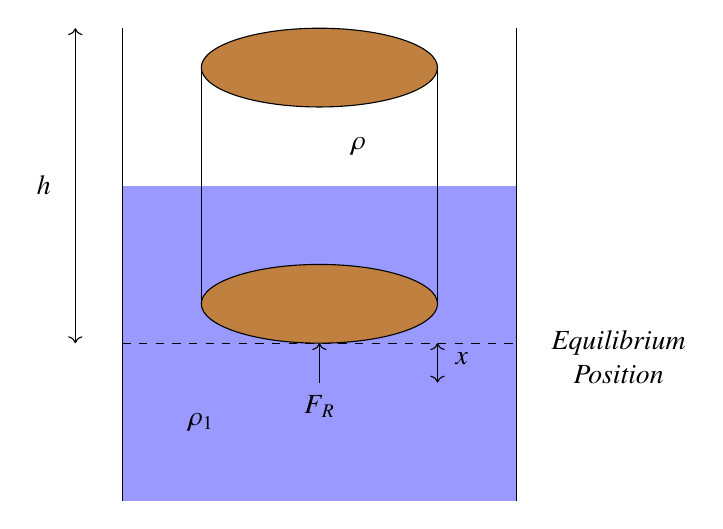
\begin{tikzpicture}
\centering
\draw (0,0) -- (5,0);
\draw (0,0) -- (0,6);
\draw (5,0) -- (5,6);
\fill[blue!40] (0,0) -- (5,0) -- (5,4) -- (0,4) -- cycle;  
  \draw[fill=brown] (2.5,5.5) ellipse (1.5 and 0.5);
      \draw[fill=brown] (2.5,2.5) ellipse (1.5 and 0.5);
          % \draw[fill = brown] (-1.5,2) -- (1.5,2);
	      % \draw[fill = brown] (-1.5,-2) -- (1.5,-2);
	          \draw[fill = brown] (1,2.5) -- (1,5.5);
		       \draw[fill = brown] (4,2.5) -- (4,5.5);

		       \draw[dashed] (0,2)--(5,2);
		       \draw [<->](-0.6,2) -- (-0.6,6);
		       \node at (-1,4){$h$};
		       \node at (3,4.5) {$\rho$};
		       \node at (1,1) {$\rho_1$};
		       \draw[<->](4,2) -- (4,1.5);
		       \node at (4.3,1.8) {$x$};
		       \node at  (6.3,2) {$\textit{Equilibrium}$};
		       \node at (6.3,1.6){$\textit{Position}$};
		       \draw [->] (2.5,1.5) -- (2.5,2);
		       \node at (2.5,1.2) {$F_R$};
		       \end{tikzpicture}

     \end{figure} \\
     When we slightly displace cylindrical piece of cork by a depth $x$,
     \begin{align}
         ```````` \\
	     \implies a &= -\frac{\rho_1Ag}{m}x \label{eqn1} \\
	         a &= -\omega^2x \label{eqn2}
		 \end{align}
		 Comparing \ref{eqn1} and \ref{eqn2},
		 \begin{align}
		     \omega^2 &= \frac{\rho_1Ag}{m} = \frac{\rho_1Ag}{\rho Ah} \\
		         \implies\omega &= \sqrt{\frac{\rho_1g}{\rho h}} \\
			     T &= \frac{2\pi}{\omega} \\
			         \therefore T &= 2\pi\sqrt{\frac{h\rho}{\rho_1 g}}
				 \end{align}
				 Hence Proved.
				 \end{document}
